% A simple Line with TikZ
% Author: Christoph Gerum <gerum@informatik.uni-tuebingen.de>

\documentclass{standalone}

\usepackage{tikz}


\begin{document}

\begin{tikzpicture}
  \draw (0, 1) -- (1, 0);
\end{tikzpicture}

\begin{tikzpicture}
  \draw (0, 1) -- (1, 0) -- (0, -1);
\end{tikzpicture}

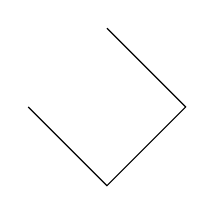
\begin{tikzpicture}
  \draw (0, 1) -- (1, 0) -- (0, -1) -- (-1, 0);
\end{tikzpicture}

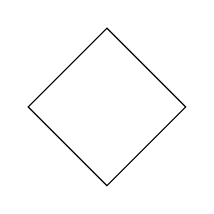
\begin{tikzpicture}
  \draw (0, 1) -- (1, 0) -- (0, -1) -- (-1, 0) -- cycle;
\end{tikzpicture}

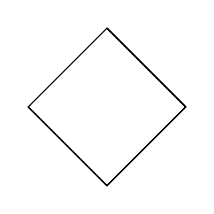
\begin{tikzpicture}
  \draw (0, 1) -- (1, 0);
  \draw (0, 1) -- (1, 0) -- (0, -1);
  \draw (0, 1) -- (1, 0) -- (0, -1) -- (-1, 0);
  \draw (0, 1) -- (1, 0) -- (0, -1) -- (-1, 0) -- cycle;
\end{tikzpicture}


\end{document}
